% !TEX TS-program = xepythontex

\documentclass[10pt, envcountsect , spanish]{beamer}


\newif\ifnotas
\notasfalse% Para no mostrar los globos
\notastrue % Para  mostrar los globos

\input ../preambulo.tex

\usepackage[normalem]{ulem}               % to striketrhourhg text
\newcommand\tacha{\bgroup\markoverwith{\textcolor{black}{\rule[0.5ex]{2pt}{0.8pt}}}\ULon}






%································ TITULO, AUTOR, ETC


\title[Excepciones y E/S]{Control de errores. Entrada y salida de datos}
\subtitle{Excepciones y E/S}

\author[L. Daniel Hernández]{L. Daniel Hernández $<ldaniel@um.es>$}

\institute[ldaniel@um.es]{Dpto. Ingeniería de la Información  y las Comunicaciones\\ Universidad de Murcia \\ 16 de noviembre de 2023\newline \hrule}


\date[ldaniel@um.es]{ 
\vskip 1.0cm
%\vskip -1.25cm
%\includegraphics[width=.8\textwidth, height=.18\textheight]{fig/polinomio}
}

\graphicspath{{img/}}






%%%%%%%%%%%%%%%%%%%%%%%%%%%%%%%%%%
%%%%%%%%%%%%%%%%%%%%%%%%%%%%%%%%%%
%%%%%%%%%%%%%%%%%%%%%%%%%%%%%%%%%%
%%%%%%%%%%%%%%%%%%%%%%%%%%%%%%%%%%

%https://es.overleaf.com/learn/how-to/Writing_Markdown_in_LaTeX_Documents
\usepackage[hashEnumerators]{markdown}


%%%%%%%%%%%%%%%%%%%%%%%%%%%%%%%%%%
%%%%%%%%%%%%%%%%%%%%%%%%%%%%%%%%%%
%%%%%%%%%%%%%%%%%%%%%%%%%%%%%%%%%%
%%%%%%%%%%%%%%%%%%%%%%%%%%%%%%%%%%
\begin{document}

%\pgfdeclareimage[height=1cm]{logo}{logo.png}
%\logo{\pgfuseimage{logo}}



%--------------------------------------------------------------------------------
{\usebackgroundtemplate{%
  \includegraphics[width=\paperwidth,height=\paperheight]{../img/fondoUMUCompleto}}

\begin{frame}[b]
	\maketitle

\begin{tikzpicture}[overlay, remember picture]
\node[anchor=south west, %anchor is bottom left corner of the graphic
      xshift=.33\textwidth, %shifting around
      yshift=0.8cm] 
     at (current page.south west) %left bottom corner of the page
     {\includegraphics[width=.5\textwidth, height=.3\textheight]{fig/java-excepciones-ejemplos}
     \footnote[frame]{\tiny
 Imagen: \url{http://puntocomnoesunlenguaje.blogspot.com/2014/04/java-excepciones.html} }}; 
\end{tikzpicture}
	
\end{frame}			% Transparencia: Título
}




%
%
%
%%%cajero.png   https://www.freepik.es/vector-gratis/elementos-cajero-automatico_959486.htm}}}
%%\mail{ivan dot valbusa at univr dot it}
%\institute[DIIC. Univ. de Murcia] % (optional)
%{
%  Departamento de Ingeniería de la Información y las Comunicaciones\\
%  Universidad de Murcia
%}
%\date{\today\ (\currenttime h)}
%\titlegraphic[width=.45\textwidth]{fig/polimorfismo}{xshift=-1.0cm, yshift=-.05\textheight}




%%%%%%%%%%%%%%%%%%%%%%%%%%%%%%%%%%%%%%%%%%%%%%%%
%%%%%%%%%%%%%%%%%%%%%%%%%%%%%%%%%%%%%%%%%%%%%%%%
\begin{frame}{Índice de Contenidos}\tableofcontents \end{frame}






%%%%%%%%%%%%%%%%%%%%%%%%%%%%%%%%%%%%%
%%%%%%%%%%%%%%%  SECTION   %%%%%%%%%%%%%%%
%%%%%%%%%%%%%%%%%%%%%%%%%%%%%%%%%%%%%
\section{Excepciones}

%%%%%%%%%%%%%%%%%%%%%%%%%%%%%%%%%%%%%
%%%%%%%%%%%%%%%%%%%%%%%%%%%%%%%%%%%%%
\begin{frame}[fragile]{Excepción = Error} \large
\small

\begin{itemize}\setlength{\itemsep}{0pt}
\item Lo que menos le gusta a un programador son los \key{errores}

\item Considera los siguientes códigos y observa las excepciones que genera:

{\tiny
\begin{pyconsole}[][frame=single, fontsize=\tiny]
print(a)
print(55/0)
print('2' + 2)
lista = None
for i in range(2):
    print(lista[i])
    
lista = []
for i in range(2):
    print(lista[i])

\end{pyconsole}
}

\item Las excepciones incorporadas en Python en \url{https://docs.python.org/es/3/library/exceptions.html}
\end{itemize}
\end{frame}
% . . . . . . . . . . . . . . . . . . . . . . . . . . . . . . . . . . . . . . . . . . . . . . . . . . . . . . 
% . . . . . . . . . . . . . . . . . . . . . . . . . . . . . . . . . . . . . . . . . . . . . . . . . . . . . . 





%%%%%%%%%%%%%%%%%%%%%%%%%%%%%%%%%%%%%
%%%%%%%%%%%%%%%%%%%%%%%%%%%%%%%%%%%%%
\begin{frame}[fragile]{Objetos de Excepciones} 

\begin{itemize}

\item Los errores \textbf{en tiempo de ejecución} se manejan usando \key{excepciones}.

\item \key{Las excepciones son objetos} que se crean cuando el programa hace algo que se considera irregular.

\item En los ejemplos anteriores cada  \textcolor{red}{xxxxError} indica que se ha creado un objeto-error.

\item Como objetos, siguen una jerarquía de clases. 

\item En Python, los usuales son las subclases de \key[red]{Exception}: !`!`Leelos!!  \\
\url{https://docs.python.org/es/3/library/exceptions.html#exception-hierarchy}

\item Cuando se crea una excepción, se dice que se ha \key{``lanzado''} una excepción.

\begin{itemize}
\item En Java lo llaman \cm{throw} (lanzar, arrojar). 
\item En Python lo llaman \cm{raise} (elevar, levantar).
\end{itemize}


\item Para tratar conveniente el error, la excepción debe ser \key{``atrapada''}

\item \textbf{Estudiaremos} cómo 
\begin{itemize}
\item Capturar excepciones
\item Lanzar/Elevar excepciones
\item Crear nuestros propios objetos excepción
\end{itemize}

\end{itemize}
\end{frame}
% . . . . . . . . . . . . . . . . . . . . . . . . . . . . . . . . . . . . . . . . . . . . . . . . . . . . . . 
% . . . . . . . . . . . . . . . . . . . . . . . . . . . . . . . . . . . . . . . . . . . . . . . . . . . . . . 




%%%%%%%%%%%%%%%%%%%%%%%%%%%%%%%%%%%%%
%%%%%%%%%%%%%%%  SECTION   %%%%%%%%%%%%%%%
%%%%%%%%%%%%%%%%%%%%%%%%%%%%%%%%%%%%%
\subsection{Capturar Excepciones}

%%%%%%%%%%%%%%%%%%%%%%%%%%%%%%%%%%%%%
%%%%%%%%%%%%%%%%%%%%%%%%%%%%%%%%%%%%%
\begin{frame}[fragile]{Capturar excepciones} 

\begin{itemize}

\item Para manejar excepciones se usan la sentencias \cm{try/except/else/finally}

\begin{pyverbatim}[][frame=single, fontsize=\scriptsize]
try:

  // Código que se desea ejecutar
  
except [zzzError [as nombre]]: 
 
  // Código a ejecutar si se produce un error en try
  // Código que controla la situación de error. Puede lanzar otro error.
  
else:

  // Bloque a ajecutar si try no tuvo errores
  
finally:

  // Código que se ejecutará siempre. Ocurra lo que ocurra en el programa.
  // P.e. cerrar los recursos
\end{pyverbatim}

\end{itemize}
\end{frame}
% . . . . . . . . . . . . . . . . . . . . . . . . . . . . . . . . . . . . . . . . . . . . . . . . . . . . . . 
% . . . . . . . . . . . . . . . . . . . . . . . . . . . . . . . . . . . . . . . . . . . . . . . . . . . . . . 


%%%%%%%%%%%%%%%%%%%%%%%%%%%%%%%%%%%%%
%%%%%%%%%%%%%%%%%%%%%%%%%%%%%%%%%%%%%
\begin{frame}[fragile]{Ejemplo de Captura de Excepciones}{\tt try/except/finally}

\unEjemplo 

\footnotesize

\begin{itemize}
\item Veamos antes el error sin capturas.
\begin{pyconsole}[][frame=single, fontsize=\scriptsize]
print(un_mensaje) 

\end{pyconsole}

\item Con las 3 componentes; pero a \cm{except} le da el igual el error.

\begin{pyconsole}[][frame=single, fontsize=\scriptsize]
try:
    print(un_mensaje)  # Código que se desea ejecutar
except:                # Salvo que se genere una excepción. Observa la salida !!
    print('Opppss ... hubo un error')   # No importa el error
finally:               # Siempre se puede obligar a cierto código
    print('Siempre muestro este mensaje')

\end{pyconsole}

\end{itemize}
\end{frame}
% . . . . . . . . . . . . . . . . . . . . . . . . . . . . . . . . . . . . . . . . . . . . . . . . . . . . . . 
% . . . . . . . . . . . . . . . . . . . . . . . . . . . . . . . . . . . . . . . . . . . . . . . . . . . . . . 

%%%%%%%%%%%%%%%%%%%%%%%%%%%%%%%%%%%%%
%%%%%%%%%%%%%%%%%%%%%%%%%%%%%%%%%%%%%
\begin{frame}[fragile]{Ejemplo de Captura de Excepciones}{\tt try/except}
\unEjemplo 
\small

\begin{itemize}

\item \cm{except} solo se activa si el error es \cm[red]{NameError}.
\begin{pyconsole}[][frame=single, fontsize=\scriptsize]
try:
    print(un_mensaje)  # Código que se desea ejecutar
except NameError:                # Salvo que se genere una excepción
    print('Opppss ... hubo un error')

\end{pyconsole}



\item \cm{except} asigna el error a una variable para poder ser manipulado.

\begin{pyconsole}[][frame=single, fontsize=\scriptsize]
try:
    print(un_mensaje)  # Código que se desea ejecutar
except NameError as error: # Salvo que se genere una excepción
    print(f'Opppss ... hubo un "{error}"')

\end{pyconsole}

\end{itemize}
\end{frame}
% . . . . . . . . . . . . . . . . . . . . . . . . . . . . . . . . . . . . . . . . . . . . . . . . . . . . . . 
% . . . . . . . . . . . . . . . . . . . . . . . . . . . . . . . . . . . . . . . . . . . . . . . . . . . . . . 




%%%%%%%%%%%%%%%%%%%%%%%%%%%%%%%%%%%%%
%%%%%%%%%%%%%%%%%%%%%%%%%%%%%%%%%%%%%
\begin{frame}[fragile]{Ejemplo de Captura de Excepciones con {\tt else}}
{\url{https://www.programiz.com/python-programming/exception-handling}}
\small
\hfil \begin{minipage}{.7\textwidth}
\begin{pyconsole}[][frame=single, fontsize=\scriptsize]
def funcion(num):
  try:
    print(f"Número introducido {num}")
    assert num % 2 == 0
  except:  # Si try SÍ ha generado excepciones
    print("No es un número par")
  else:    # Si try NO ha generado excepciones
    reciproco = 1/num
    print(reciproco)
    
\end{pyconsole}    
\end{minipage}

\begin{itemize}

\item Se activa \cm{except}
\begin{pyconsole}[][frame=single, fontsize=\scriptsize]
funcion(1)
    
\end{pyconsole}   



\item Se activa \cm{else}

\begin{pyconsole}[][frame=single, fontsize=\scriptsize]
funcion(4)
    
\end{pyconsole}   

\end{itemize}
\end{frame}
% . . . . . . . . . . . . . . . . . . . . . . . . . . . . . . . . . . . . . . . . . . . . . . . . . . . . . . 
% . . . . . . . . . . . . . . . . . . . . . . . . . . . . . . . . . . . . . . . . . . . . . . . . . . . . . . 




%%%%%%%%%%%%%%%%%%%%%%%%%%%%%%%%%%%%%
%%%%%%%%%%%%%%%%%%%%%%%%%%%%%%%%%%%%%
\begin{frame}[fragile]{Varios {\tt except}} 

\begin{itemize}

\item Si se conoce la jerarquía de clases de las excepciones se pueden usar varios \mbox{``\cm{except}''}.

\item Las capturas ``\cm{except}'' se ordenarán desde las subclases a las superclases



\item Código correcto.
{\scriptsize
\begin{pyconsole}[][frame=single, fontsize=\scriptsize]
try:
    print(100/0)
except ZeroDivisionError:   #  ZeroDivisionError es SUBclase de ArithmeticError
    print("Error: divides por cero")
except ArithmeticError:
    print("Error aritmético")

\end{pyconsole}
}

\item Código incorrecto
{\scriptsize
\begin{pyconsole}[][frame=single, fontsize=\scriptsize]
try:
    print(100/0)
except ArithmeticError:   #  ArithmeticError es una SUPERclase de ZeroDivisionError 
    print("Error aritmético")
except ZeroDivisionError:
    print("Error: divides por cero")

\end{pyconsole}
}

Nunca se capturará un objeto de {\tt \color{red} ZeroDivisionError}.
\end{itemize}

\end{frame}
% . . . . . . . . . . . . . . . . . . . . . . . . . . . . . . . . . . . . . . . . . . . . . . . . . . . . . . 
% . . . . . . . . . . . . . . . . . . . . . . . . . . . . . . . . . . . . . . . . . . . . . . . . . . . . . . 






%%%%%%%%%%%%%%%%%%%%%%%%%%%%%%%%%%%%%
%%%%%%%%%%%%%%%  SECTION   %%%%%%%%%%%%%%%
%%%%%%%%%%%%%%%%%%%%%%%%%%%%%%%%%%%%%
\subsection{Lanzar Excepciones}

%%%%%%%%%%%%%%%%%%%%%%%%%%%%%%%%%%%%%
%%%%%%%%%%%%%%%%%%%%%%%%%%%%%%%%%%%%%
\begin{frame}[fragile]{Lanzar excepciones} 

\begin{itemize}
\item El programador también puede crear excepciones

\item El programador puede \key{lanzar una excepcion} utilizando \cm{raise} o  \cm{assert}.

\item[]\unEjemplo Para indicar que un método aún no ha sido implementado.

\begin{pyconsole}[][frame=single, fontsize=\scriptsize]
def metodo():
    raise NotImplementedError("Not supported yet.")

metodo()

\end{pyconsole}

\item[]\unEjemplo Para indicar que un parámetro no es el adecuado.

\begin{columns}
\begin{column}{.48\textwidth}
\begin{pyconsole}[][frame=single, fontsize=\tiny]
def metodo(param):
 assert param > 0, "Deber ser positivo"

metodo(-1)

\end{pyconsole}
\end{column}

\begin{column}{.48\textwidth}
\begin{pyconsole}[][frame=single, fontsize=\tiny]
def metodo(param):
 if param <= 0:
  raise ValueError("Deber ser positivo")

metodo(-1)

\end{pyconsole}
\end{column}
\end{columns}

\end{itemize}
\end{frame}
% . . . . . . . . . . . . . . . . . . . . . . . . . . . . . . . . . . . . . . . . . . . . . . . . . . . . . . 
% . . . . . . . . . . . . . . . . . . . . . . . . . . . . . . . . . . . . . . . . . . . . . . . . . . . . . . 




%%%%%%%%%%%%%%%%%%%%%%%%%%%%%%%%%%%%%
%%%%%%%%%%%%%%%%%%%%%%%%%%%%%%%%%%%%%
\begin{frame}[fragile]{Excepciones en Setter/Propiedades} 

\begin{itemize}
\item La interface Setter permite asignar valores a los atributos de instancia de una clase.

\item Los métodos Setter de una atributo deben lanzar errores/excepciones cuando los valores a asignar sean incorrectos.



\item Alternativamente, se puede usar propiedades.



{\footnotesize
Mira \url{https://realpython.com/python-property/#putting-pythons-property-into-action} para usar property con raise.
}


\item[]\unEjemplo Para indicar que un valor debe ser entero positivo.

\begin{pyverbatim}[][frame=single, fontsize=\scriptsize]
class Dia:
    def __init__(self, d: int):
        self._dia = d
    @property
    def dia(self):
        return self._dia
    @dia.setter
    def dia(self, valor: int):
        try:
            self._dia = int(valor)
            assert self._dia > 0
        except Exception as e:
            print(f"#ERROR {e.__class__}")
            
\end{pyverbatim}

\end{itemize}
\end{frame}
% . . . . . . . . . . . . . . . . . . . . . . . . . . . . . . . . . . . . . . . . . . . . . . . . . . . . . . 
% . . . . . . . . . . . . . . . . . . . . . . . . . . . . . . . . . . . . . . . . . . . . . . . . . . . . . . 






%%%%%%%%%%%%%%%%%%%%%%%%%%%%%%%%%%%%%
%%%%%%%%%%%%%%%  SECTION   %%%%%%%%%%%%%%%
%%%%%%%%%%%%%%%%%%%%%%%%%%%%%%%%%%%%%
\subsection{Definir Excepciones del Usuario}

%%%%%%%%%%%%%%%%%%%%%%%%%%%%%%%%%%%%%
%%%%%%%%%%%%%%%%%%%%%%%%%%%%%%%%%%%%%
\begin{frame}[fragile]{Creando Excepciones Nuevas} 

\begin{itemize}
\item Pueden crearse subclases a partir de la clase \cm{Exception}
\item Usa la notación usual de creación: \pyv{class MiError(Excepcion)}

{\footnotesize
\begin{pyconsole}[][frame=single, fontsize=\scriptsize]
class BaseError(Exception):
  """Mi clase base para mis excepciones"""
  pass  # Lo correcto es definir __init__(self, *args)
  
raise BaseError   # Alza un error sin texto
\end{pyconsole}
}

\item Se pueden construir clases hijas: \pyv{class ConcretoError(MiError)}


{\footnotesize
\begin{pyconsole}[][frame=single, fontsize=\scriptsize]
class ConcretoError(BaseError):
  """Una clase concreta para mis excepciones"""
  pass   # Lo correcto es definir __init__(self, *args)
  
raise ConcretoError("Esto es un error concreto")  # Con texto
\end{pyconsole}
}

\item Es una buena práctica colocar todas las excepciones en algún fichero separado como \key[orange]{exceptions.py} o \key[orange]{errors.py}. Pero esto no es obligatorio.

\end{itemize}
\end{frame}
% . . . . . . . . . . . . . . . . . . . . . . . . . . . . . . . . . . . . . . . . . . . . . . . . . . . . . . 
% . . . . . . . . . . . . . . . . . . . . . . . . . . . . . . . . . . . . . . . . . . . . . . . . . . . . . . 






%%%%%%%%%%%%%%%%%%%%%%%%%%%%%%%%%%%%%
%%%%%%%%%%%%%%%%%%%%%%%%%%%%%%%%%%%%%
\begin{frame}[fragile]{Personalizando las Excepciones Nuevas} 

\begin{itemize}
\item Las nuevas clases, como cualquier otra, pueden tener su propio constructor y métodos.
\item Esto nos permite crear excepciones más personalizadas.
\end{itemize}
{\footnotesize
\begin{pyconsole}[][frame=single, fontsize=\scriptsize]
class NotInRangeError(Exception):
  def __init__(self, valor: int, mensaje="No está en el rango (10, 40)"):
    self._valor = valor
    self._mensaje = str(valor) + " -> " + mensaje
    super().__init__(self._mensaje)

valor = 50
if valor < 10 or 40 < valor:
  raise NotInRangeError(valor)
    
\end{pyconsole}
}


\end{frame}
% . . . . . . . . . . . . . . . . . . . . . . . . . . . . . . . . . . . . . . . . . . . . . . . . . . . . . . 
% . . . . . . . . . . . . . . . . . . . . . . . . . . . . . . . . . . . . . . . . . . . . . . . . . . . . . . 




%%%%%%%%%%%%%%%%%%%%%%%%%%%%%%%%%%%%%
%%%%%%%%%%%%%%%%%%%%%%%%%%%%%%%%%%%%%
\begin{frame}{Ejercicio} 

\begin{ejercicio}{}

\setlist[itemize,1]{before*=\normalsize, leftmargin=\dimexpr 8pt}%,label=$\triangleleft$}

\begin{itemize}
\item Crea la clase \cm{SintaxisError} y sus subclases \cm{SinArrobaSintaxisError} y \cm{CadenaVaciaSintaxisError} 

\item Sobre la clase \cm{Persona} se tienen los atributos \cm{eMail} y  \cm{nombre}.

\item Se quieren detectar los errores de que el correo electrónico no tiene arroba \cm{@} y que el nombre dado no es ni nulo ni tiene una longitud inferior a 3 caracteres.

\item Escribe las clases indicadas con sus constructores, que deberán de lanzar las correspondientes excepciones si fuera necesario.

\item Escribe el programa para una prueba unitaria
\end{itemize}

\end{ejercicio}

\end{frame}
% . . . . . . . . . . . . . . . . . . . . . . . . . . . . . . . . . . . . . . . . . . . . . . . . . . . . . . 
% . . . . . . . . . . . . . . . . . . . . . . . . . . . . . . . . . . . . . . . . . . . . . . . . . . . . . . 






%%%%%%%%%%%%%%%%%%%%%%%%%%%%%%%%%%%%%
%%%%%%%%%%%%%%%  SECTION   %%%%%%%%%%%%%%%
%%%%%%%%%%%%%%%%%%%%%%%%%%%%%%%%%%%%%
\section{Entrada y Salida de Datos}



%%%%%%%%%%%%%%%%%%%%%%%%%%%%%%%%%%%%%
%%%%%%%%%%%%%%%%%%%%%%%%%%%%%%%%%%%%%
\begin{frame}{Entrada y Salida} 
\begin{itemize}
\item Un \key{stream} (secuencia o flujo) es  una representación abstracta de un dispositivo físico de entrada o salida. 

\item Un stream \textbf{puede imaginarse} como un tubo por el que fluyen bytes de datos y dónde una vez transmitido el dato éste no se volverá a enviar.

\item Hay \key{dos tipos de flujos} atendiendo a ``su dirección'': 
\begin{itemize}
\item Flujos de \textbf{entrada}: teclado, archivo de disco, ...
\item Flujos de \textbf{salida}: archivo de disco, una consola, impresora ...
\end{itemize}

\item En Python se distinguen los siguientes tipos:
\begin{itemize}
\item \key{E/S de texto.} En el flujo los datos serán objetos de la clase \key{str}.

Representa los objetos como cadena de caracteres.

\item \key{E/S binario} (o \textit{buffered I/O}). En el flujo se esperan objetos de tipo binario y produce objetos de tipo \key{bytes}.

\begin{itemize}
\item Algunos objetos de tipo binarios son \key{bytes}, \key{bytearray}, \key{array.array}, etc ...
\item El tratamiento básico de los objetos \key{bytes} es como una secuencia  de números enteros y cada uno restringido a valores $x$ con $0\leq x\< 256$.
\item Los valores literales de \key{bytes} son igual que la cadenas de texto anteponiendo la letra \key{b}.
	\unEjemplo \pyv{"hola"} es un str,  \pyv{b"hola"} es un bytes.
\end{itemize}



\item \key{E/S sin formato} (o \textit{unbuffered I/O}). Trata los datos en crudo, a bajo nivel, no hace ningún tipo de encapsulación (agrupamiento).
\end{itemize}

\end{itemize}
\end{frame}
% . . . . . . . . . . . . . . . . . . . . . . . . . . . . . . . . . . . . . . . . . . . . . . . . . . . . . . 
% . . . . . . . . . . . . . . . . . . . . . . . . . . . . . . . . . . . . . . . . . . . . . . . . . . . . . . 





%%%%%%%%%%%%%%%%%%%%%%%%%%%%%%%%%%%%%
%%%%%%%%%%%%%%%  SECTION   %%%%%%%%%%%%%%%
%%%%%%%%%%%%%%%%%%%%%%%%%%%%%%%%%%%%%
\subsection{Entrada y Salida Estándar}

%%%%%%%%%%%%%%%%%%%%%%%%%%%%%%%%%%%%%
%%%%%%%%%%%%%%%%%%%%%%%%%%%%%%%%%%%%%
\begin{frame}[fragile]{Entrada y Salida Estándar.} 
\begin{itemize}
\item Se trabaja con \key{E/S de texto.}

\item \textbf{Mostrar objetos en la pantalla.}\\
{ \pyv{print(*objects, sep=' ', end='\n', file=sys.stdout, flush=False)}}



\begin{itemize}
\item Todos los argumentos de \cm{*objects} se convierten a cadenas de caracteres.
\item Los objetos se mandan al flujo separados por  \cm{sep}.
\item Se termina el envío con  \cm{end}.
\item \cm{file} debe ser un objeto que implemente un método \cm{write(string)}.

Si no se indica se usará  \key{sys.stdout}.
También puede usar  \key{sys.stderr} (donde se envían las indicaciones del intérprete y mensajes de error).

\item \cm{flush} indica si se obliga a vaciar el buffer del stream.
\end{itemize}


\item \textbf{Lee datos del teclado.}  \pyv{input([prompt])}


\begin{itemize}
\item Si se indica \cm{prompt} se mostrará en la salida estándar sin nueva línea.

\item Lee  una línea de la entrada \key{sys.stdin}, la convierte en una cadena (eliminando la nueva línea), y retorna eso.
\end{itemize}

\end{itemize}

\begin{pyverbatim}[][frame=single, fontsize=\scriptsize]
>>> s=input("Dime tu edad: ")
Dime tu edad: 22
>>> print(f"{'Sí' if int(s)>17 else 'No'} eres mayor de edad")
Sí eres mayor de edad
\end{pyverbatim}
\end{frame}
% . . . . . . . . . . . . . . . . . . . . . . . . . . . . . . . . . . . . . . . . . . . . . . . . . . . . . . 
% . . . . . . . . . . . . . . . . . . . . . . . . . . . . . . . . . . . . . . . . . . . . . . . . . . . . . . 



%%%%%%%%%%%%%%%%%%%%%%%%%%%%%%%%%%%%%
%%%%%%%%%%%%%%%%%%%%%%%%%%%%%%%%%%%%%
\begin{frame}[fragile]{Formatear Cadenas} 
\begin{itemize}
\item \key{Formatear cadenas de texto}: cambiar la salida (texto) de un programa para que sea legible por humanos, incluyendo texto y datos.

\item Python ofrece \textbf{dos formas} para realizar el formato.

\item Usar el \key{método} \cm{str.format() }
\begin{itemize}
\item \cm{str} contienen campos de reemplazo, que son expresiones delimitadas por llaves \cm{\{\}}
\end{itemize}

{\small
\begin{pyconsole}[][frame=single, fontsize=\scriptsize]
for x in range(1, 3):
  print("'{0}' {2:10} {1:10.2f}".format(repr(x), x, x*x))
 
\end{pyconsole}
}

\item \textbf{Literales de cadena formateados} (formatted string literal o \key{f-string}). 
\begin{itemize}
\item Es un literal de cadena que  prefijo  'f' o 'F'. 
\item Contienen campos de reemplazo, que son expresiones delimitadas por llaves \cm{\{\}}
\end{itemize}

{\small
\begin{pyconsole}[][frame=single, fontsize=\scriptsize]
for x in range(1, 3):
  print(f"{str(x)!r:10} {x*x: 8d} {x: 10.2f}")
 
\end{pyconsole}
}

\tiny \url{https://docs.python.org/es/3/reference/lexical_analysis.html#f-strings}
\end{itemize}

\end{frame}
% . . . . . . . . . . . . . . . . . . . . . . . . . . . . . . . . . . . . . . . . . . . . . . . . . . . . . . 
% . . . . . . . . . . . . . . . . . . . . . . . . . . . . . . . . . . . . . . . . . . . . . . . . . . . . . . 

%%%%%%%%%%%%%%%%%%%%%%%%%%%%%%%%%%%%%
%%%%%%%%%%%%%%%  SECTION   %%%%%%%%%%%%%%%
%%%%%%%%%%%%%%%%%%%%%%%%%%%%%%%%%%%%%
\subsection{Entrada y Salida a Ficheros}


%%%%%%%%%%%%%%%%%%%%%%%%%%%%%%%%%%%%%
%%%%%%%%%%%%%%%%%%%%%%%%%%%%%%%%%%%%%
\begin{frame}{Esquema General}{Pasos a seguir siempre}

%\noindent Cuando se usa un fichero siempre se siguen los siguientes pasos:

\setlist[enumerate, 1]{label*=\arabic*., leftmargin=\dimexpr 26pt-.4in, listparindent=0pt, font=\bfseries\normalsize, before*=\normalsize }
\setlist[itemize,1]{before*=\small, leftmargin=\dimexpr 5pt}%,label=$\triangleleft$}


\begin{enumerate}
\item \key{Abrir un fichero.} \pyv{f = open(file, mode='r')}
	\begin{itemize}
	\item 
	\key{file} es un string indicando la ubicación del fichero.
	
	\item 
	\key{mode} es el modo de E/S. Por defecto es de lectura con flujo de texto.
	
	\item 
	Retorna un \key{file object}, que tiene una interface para tratar archivos (pasos siguientes) junto con algunos  atributos:
		\begin{itemize}
		
		\item 
		\pyv{f.closed}: True si el fichero está cerrado. Falso en otro caso.
		
		\item 
		\pyv{f.mode}: Indica el modo de acceso de cómo se abrió el fichero.
		
		\item 
		\pyv{f.name}: Indica el nombre del fichero.
		
		\end{itemize}
	\end{itemize}
	
\item \key{Leer/Escribir en el fichero.}

	\begin{itemize}
	\item 
	\pyv{f.write(string)}: Escribe un string en el fichero abierto.
	
	\item 
	\pyv{f.read([n])}: Vuelca en un string el contenido del fichero abierto.
	Opcionalmente se puede indicar el número de bytes que se quieran leer.
	
	\item 
	\pyv{f.readline()}: Lee una sola línea del archivo.
	Deja \pyv{\n} al final de la cadena. 
	
	\item 
	\pyv{f.readlines()}: Vuelca en una lista de strings el contenido del fichero
		
	\item 
	\pyv{f.writelines(lista)}: Escribe una lista de  líneas en el archivo.
	
	\item
	\pyv{f.tell()}: Indica la posición actual del puntero.
	
	\item 
	\pyv{f.seek(offset[, from])}: Cambia la posición según offset desde una posición dada. 
	Si \texttt{from} es 0 indica el inicio, 1 indica la posición actual y 2 indica la posición final.
	
	\end{itemize}
	
\item \key{Cerrar el fichero.}

	\begin{itemize}
	
	\item
	\pyv{f.close()}: Cierra el fichero
	
	\end{itemize}
\end{enumerate}

\end{frame}

%%%%%%%%%%%%%%%%%%%%%%%%%%%%%%%%%%%%%
%%%%%%%%%%%%%%%%%%%%%%%%%%%%%%%%%%%%%
\begin{frame}{Modos de Apertura} 

\begin{columns}

\begin{column}{.79\textwidth}
\setlist[itemize,1]{before*=\small, leftmargin=\dimexpr 5pt}%,label=$\triangleleft$}

\begin{itemize}
\item Un fichero se puede \key{leer}, se puede \key{sobreescibir} sobre él o hacer \key{las dos cosas} simultáneamente.

\item A la vez, la E/S puede ser de \key{texto} o \key{binaria}.

\item Python usa varios indicadores para eso.

\item\key{ r}: Abre el fichero para \textbf{lectura}. El fichero debe existir. El puntero del fichero se coloca al \textbf{principio}. Este modo es por defecto.
\item \key{w}: Abre el fichero para \textbf{escritura}. Sobreescribe el fichero si existe. El puntero del fichero se coloca al \textbf{principio}. 
\item \key{a}: Abre el fichero para \textbf{añadir}. Si no existe el fichero lo crea. Si existe, coloca el puntero del fichero al \textbf{final}.

\end{itemize}

\end{column}

\begin{column}{.19\textwidth}
\tikzset{every picture/.style={line width=0.75pt}} %set default line width to 0.75pt        

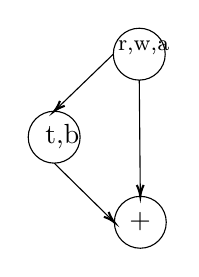
\begin{tikzpicture}[x=0.75pt,y=0.75pt,yscale=-0.5,xscale=0.5]
%uncomment if require: \path (0,380); %set diagram left start at 0, and has height of 380

%Shape: Circle [id:dp33266581686988106] 
\draw   (261,85) .. controls (261,71.19) and (272.19,60) .. (286,60) .. controls (299.81,60) and (311,71.19) .. (311,85) .. controls (311,98.81) and (299.81,110) .. (286,110) .. controls (272.19,110) and (261,98.81) .. (261,85) -- cycle ;
%Shape: Circle [id:dp021356845102042277] 
\draw   (179,165) .. controls (179,151.19) and (190.19,140) .. (204,140) .. controls (217.81,140) and (229,151.19) .. (229,165) .. controls (229,178.81) and (217.81,190) .. (204,190) .. controls (190.19,190) and (179,178.81) .. (179,165) -- cycle ;
%Shape: Circle [id:dp3917157457183982] 
\draw   (262,247) .. controls (262,233.19) and (273.19,222) .. (287,222) .. controls (300.81,222) and (312,233.19) .. (312,247) .. controls (312,260.81) and (300.81,272) .. (287,272) .. controls (273.19,272) and (262,260.81) .. (262,247) -- cycle ;
%Straight Lines [id:da857735408573197] 
\draw    (286,110) -- (286.98,220) ;
\draw [shift={(287,222)}, rotate = 269.49] [color={rgb, 255:red, 0; green, 0; blue, 0 }  ][line width=0.75]    (10.93,-3.29) .. controls (6.95,-1.4) and (3.31,-0.3) .. (0,0) .. controls (3.31,0.3) and (6.95,1.4) .. (10.93,3.29)   ;
%Straight Lines [id:da6253239937628281] 
\draw    (204,190) -- (260.57,245.6) ;
\draw [shift={(262,247)}, rotate = 224.5] [color={rgb, 255:red, 0; green, 0; blue, 0 }  ][line width=0.75]    (10.93,-3.29) .. controls (6.95,-1.4) and (3.31,-0.3) .. (0,0) .. controls (3.31,0.3) and (6.95,1.4) .. (10.93,3.29)   ;
%Straight Lines [id:da5061303295781583] 
\draw    (261,85) -- (205.44,138.61) ;
\draw [shift={(204,140)}, rotate = 316.02] [color={rgb, 255:red, 0; green, 0; blue, 0 }  ][line width=0.75]    (10.93,-3.29) .. controls (6.95,-1.4) and (3.31,-0.3) .. (0,0) .. controls (3.31,0.3) and (6.95,1.4) .. (10.93,3.29)   ;

% Text Node
\draw (263,70) node [anchor=north west][inner sep=0.75pt]  [font=\footnotesize] [align=left] {r,w,a};
% Text Node
\draw (193,150) node [anchor=north west][inner sep=0.75pt]   [align=left] {t,b};
% Text Node
\draw (274,235) node [anchor=north west][inner sep=0.75pt]  [align=left] {+};

\end{tikzpicture}
\end{column}

\end{columns}

\setlist[itemize,1]{before*=\small, leftmargin=\dimexpr 0pt}%,label=$\triangleleft$}

\begin{itemize}
\item \key{b}: Si se especifica se tratará el fichero como \textbf{binario}. 

\item \key{t}: Será una E/S de texto. Valor por defecto.

\item \key{+}:  Se puede usar el fichero para \textbf{leer y escribir}.

\item \key{x}:  Abierto para \textbf{creación} en exclusiva, falla si el fichero ya existe.
\end{itemize}

\hskip-0.5cm\unEjemplo

\begin{itemize}
\item \key{rb+}: Para leer. Puntero al principio. Será una E/S binaria. También se podrá escribir.
\item \key{a+}: Para añadir. Puntero al final. Será una E/S texto. También se podrá leer.
\end{itemize}

\end{frame}
% . . . . . . . . . . . . . . . . . . . . . . . . . . . . . . . . . . . . . . . . . . . . . . . . . . . . . . 
% . . . . . . . . . . . . . . . . . . . . . . . . . . . . . . . . . . . . . . . . . . . . . . . . . . . . . . 




%%%%%%%%%%%%%%%%%%%%%%%%%%%%%%%%%%%%%
%%%%%%%%%%%%%%%%%%%%%%%%%%%%%%%%%%%%%
\begin{frame}[fragile]{Ejemplos Básicos} 

\begin{pyverbatim}[][frame=single]%, fontsize=\scriptsize]

# Crear un fichero y escribe 3 líneas
f = open("test.txt", "w")
for num in range(3):
  f.write(str(num)+'\n') # \n para nueva línea
f.close()

# Lo abre de nuevo para añadir una cuarta línea
f = open("test.txt", "a")
f.write(str(4)+'\n')
f.close()

# Mostramos el contenido en pantalla
f = open("test.txt")
for linea in f:
  print(linea)
f.seek(0)  # Para empezar desde el principio
lista= f.readlines()
f.close()
\end{pyverbatim}

\end{frame}



%%%%%%%%%%%%%%%%%%%%%%%%%%%%%%%%%%%%%
%%%%%%%%%%%%%%%%%%%%%%%%%%%%%%%%%%%%%
\begin{frame}[fragile]{Ficheros con {\tt try/excepts}} 

\begin{itemize}
\item Si no existe el fichero para una lectura se  generará un error.
{\small
\begin{pyconsole}[][frame=single]%, fontsize=\scriptsize]

f = open("testR.txt")
\end{pyconsole}
}

\item En estos casos se debe usar try/excepts
{\small
\begin{pyconsole}[][frame=single]%, fontsize=\scriptsize]

try:
  f = open("testR.txt")
except:
  print("Opppps ! ... y no se cierra el fichero.") 
else:
  f.read()
  f.close()
  print("Tarea realizada con éxito")
  
\end{pyconsole}
}
\end{itemize}

\end{frame}







%%%%%%%%%%%%%%%%%%%%%%%%%%%%%%%%%%%%%
%%%%%%%%%%%%%%%%%%%%%%%%%%%%%%%%%%%%%
\begin{frame}[fragile]{Ficheros con {\tt with}} 

\begin{itemize}
\item Es importante que no se generen errores ANTES de cerrar el fichero
{\small
\begin{pyconsole}[][frame=single]%, fontsize=\scriptsize]

f = open("testW.txt", "w")
f.read()
print(f"Está cerrado? {f.closed}")
\end{pyconsole}
}

\item \key{Es fundamental cerrar el fichero}\cm{ f.close()}

\item Python garantiza el cierre usando \cm{with}
{\small
\begin{pyconsole}[][frame=single]%, fontsize=\scriptsize]

try:
  with open("testW.txt", "w") as f:
    f.read()            # Genera error, pero se cerrará
except:
  print(f"Está cerrado? {f.closed}")

\end{pyconsole}
}

Notar que no se usa \cm{f.close()} en el código anterior.
\end{itemize}

\end{frame}



%%%%%%%%%%%%%%%%%%%%%%%%%%%%%%%%%%%%%
%%%%%%%%%%%%%%%%%%%%%%%%%%%%%%%%%%%%%
\begin{frame}[fragile]{Algo más sobre la sentencia {\tt with}} 

\begin{columns}

\begin{column}{.73\textwidth}
\begin{itemize}
\item \cm{with} genera un \key{Administrador de Contexto.}
\item Un Administrador de Contexto \key{es un objeto que maneja la entrada y salida del contexto} para la ejecución del código que se indique en el bloque (BLOCK).
\end{itemize}
\end{column}

\begin{column}{.24\textwidth}
{\small
\begin{pyverbatim}[][frame=single, fontsize=\scriptsize]
with EXPR as VAR:
    BLOCK

\end{pyverbatim}
}
\end{column}

\end{columns}



\begin{itemize}
\item EXPR es la expresión que \key{define} el Administrador de Contexto.
\item VAR es un objeto de asignación.
\item Ejemplos en distintos contextos

\begin{columns}

\begin{column}{.42\textwidth}
{\footnotesize
\begin{pyverbatim}[][frame=single, fontsize=\scriptsize]
# Abrir un fichero y manipularlo
with open('text.txt', 'r') as f:
  # Block
\end{pyverbatim}
}
\end{column}


\begin{column}{.58\textwidth}
{\footnotesize
\begin{pyverbatim}[][frame=single, fontsize=\scriptsize]
# Abrir una base de datos y dar una respuesta
with sqlite3.connect('test.db') as connection:
  # Block
\end{pyverbatim}
}
\end{column}

\end{columns}

\item Se puede crear un Administrador de Contexto en una clase con los métodos \pyv{__enter__()} and \pyv{__exit__()}.

\tiny 
\begin{columns}

\begin{column}{.5\textwidth}

\begin{pyverbatim}[][frame=single, fontsize=\tiny]
def __enter__(self):
  self.file_handler = open(self.file_name, self.mode)
  return self.file_handler
\end{pyverbatim}

\end{column}


\begin{column}{.45\textwidth}

\begin{pyverbatim}[][frame=single, fontsize=\tiny]
def __exit__(self, exc_type, exc_val, traceback):
  if self.file_handler:
    self.file_handler.close()
  return True
\end{pyverbatim}

\end{column}

\end{columns}

\small 
Para saber más: \url{https://realpython.com/python-with-statement/}
\end{itemize}

\end{frame}





%%%%%%%%%%%%%%%%%%%%%%%%%%%%%%%%%%%%%
%%%%%%%%%%%%%%%  SECTION   %%%%%%%%%%%%%%%
%%%%%%%%%%%%%%%%%%%%%%%%%%%%%%%%%%%%%
\subsection{Ficheros con JSON}


%%%%%%%%%%%%%%%%%%%%%%%%%%%%%%%%%%%%%
%%%%%%%%%%%%%%%%%%%%%%%%%%%%%%%%%%%%%
\begin{frame}[fragile]{JSON} 
\begin{itemize}
\item JSON (JavaScript Object Notation) es un formato ligero de intercambio de datos.

\begin{pyverbatim}
{
    "departamento": 8,
    "nombredepto": "Ventas",
    "director": "Juan Rodriguez",
    "empleados": [
        {
            "nombre": "Pedro",
            "apellido": "Fernández"
        },
        {
            "nombre": "Jacinto",
            "apellido": "Benavente"
        }
    ]
}
\end{pyverbatim}

\item En lo esencial es una diccionario cuyos valores pueden ser: (1) un valor, (2) una lista de valores, (3) una lista de diccionarios.
\end{itemize}
\end{frame}
% . . . . . . . . . . . . . . . . . . . . . . . . . . . . . . . . . . . . . . . . . . . . . . . . . . . . . . 
% . . . . . . . . . . . . . . . . . . . . . . . . . . . . . . . . . . . . . . . . . . . . . . . . . . . . . . 




%%%%%%%%%%%%%%%%%%%%%%%%%%%%%%%%%%%%%
%%%%%%%%%%%%%%%%%%%%%%%%%%%%%%%%%%%%%
\begin{frame}[fragile]{Ejemplo - I} 
Definimos en \textbf{una variable} toda la información:

\begin{pyconsole}[][frame=single]%, fontsize=\scriptsize]

empresa = {
  "departamento": 8,
  "nombredepto": "Ventas",
  "director": "Juan Rodríguez",
  "empleados": [
  {
    "nombre": "Pedro",
    "apellido": "Fernández"
  }, {
    "nombre": "Jacinto",
    "apellido": "Benavente"
  }
  ]
}
\end{pyconsole}
\end{frame}
% . . . . . . . . . . . . . . . . . . . . . . . . . . . . . . . . . . . . . . . . . . . . . . . . . . . . . . 
% . . . . . . . . . . . . . . . . . . . . . . . . . . . . . . . . . . . . . . . . . . . . . . . . . . . . . . 


%%%%%%%%%%%%%%%%%%%%%%%%%%%%%%%%%%%%%
%%%%%%%%%%%%%%%%%%%%%%%%%%%%%%%%%%%%%
\begin{frame}[fragile]{Ejemplo - II} 
\footnotesize
\begin{pyconsole}[][frame=single, fontsize=\scriptsize]
import json   # Hay que importar esta librería

with open("json.txt", "w") as f:       # Escritura texto
  json.dump(empresa, f, indent=4)

with open("json.txt", "r") as f:       # Lectura texto. Retorna un Diccionario
  empresa = json.load(f)

print(json.dumps(empresa, indent=4)) # Lo convierte a str con formato JSON

\end{pyconsole}
\end{frame}
% . . . . . . . . . . . . . . . . . . . . . . . . . . . . . . . . . . . . . . . . . . . . . . . . . . . . . . 
% . . . . . . . . . . . . . . . . . . . . . . . . . . . . . . . . . . . . . . . . . . . . . . . . . . . . . . 





%%%%%%%%%%%%%%%%%%%%%%%%%%%%%%%%%%%%%
%%%%%%%%%%%%%%%  SECTION   %%%%%%%%%%%%%%%
%%%%%%%%%%%%%%%%%%%%%%%%%%%%%%%%%%%%%
\subsection{Ficheros  con pickle}


%%%%%%%%%%%%%%%%%%%%%%%%%%%%%%%%%%%%%
%%%%%%%%%%%%%%%%%%%%%%%%%%%%%%%%%%%%%
\begin{frame}[fragile]{Serialización de objetos Python} 
\begin{itemize}
\item Los pickles de Python representan un objeto Python como una cadena de bytes.
\item Se pueden transmitir por red o guardar en un archivo.
\end{itemize}


\footnotesize
\begin{pyverbatim}[][frame=single]%, fontsize=\scriptsize]

>>> import pickle   # Hay que importar esta librería

>>> datos = [list().append(2), set().add(100)]

>>> with open("datos.pickle", "wb") as f:         # Escritura *binario*
...  pickle.dump(datos, f)
...
>>> with open("datos.pickle", "rb") as f:         # Lectura *binario*
...  datos_p = pickle.load(f)
...
>>> print(pickle.dumps(datos_p)) # Pickle como cadena binaria (bytes)
b'\x80\x04\x95\x15\x00\x00\x00\x00\x00\x00\x00]\x94(]\x94(K\x01K\x02e\x8f\x94(K\x03K\x04\x90e.'

>>> print(datos_r) # Lo convierte a str 
[[1, 2], {3, 4}]
\end{pyverbatim}
\end{frame}
% . . . . . . . . . . . . . . . . . . . . . . . . . . . . . . . . . . . . . . . . . . . . . . . . . . . . . . 
% . . . . . . . . . . . . . . . . . . . . . . . . . . . . . . . . . . . . . . . . . . . . . . . . . . . . . . 




%%%%%%%%%%%%%%%%%%%%%%%%%%%%%%%%%%%%%
%%%%%%%%%%%%%%%  SECTION   %%%%%%%%%%%%%%%
%%%%%%%%%%%%%%%%%%%%%%%%%%%%%%%%%%%%%
\subsection{Librerías}

%%%%%%%%%%%%%%%%%%%%%%%%%%%%%%%%%%%%%
%%%%%%%%%%%%%%%%%%%%%%%%%%%%%%%%%%%%%
\begin{frame}[fragile]{No reinventes la rueda} 
\hskip-0,5cm Algunas librerías para manipular ficheros.

\begin{description}
\item[csv:] Leer y escribir a ficheros .csv (Excel)
\item[xlwings:] Leer y escribir a ficheros .xls (Excel)
\item[wave:]  Leer y escribir a ficheros WAV (audio Microsoft)
\item[aifc:] Leer y escribir a ficheros AIFF y AIFC  (audio)
\item[tarfile:] Leer y escribir a ficheros tar (compresión)
\item[zipfile:] Leer y escribir a ficheros ZIP (compresión)
\item[xml.etree.ElementTree:] Leer y escribir a ficheros XML (marcas)
\item[msilib:] Leer y escribir a ficheros de instalación de Microsoft.
\item[PyPDF2:] Manipulación de ficheros .pdf (Adobe)
\item[Pillow:] Manipulación de ficheros de imágenes.
\end{description}
\end{frame}
% . . . . . . . . . . . . . . . . . . . . . . . . . . . . . . . . . . . . . . . . . . . . . . . . . . . . . . 
% . . . . . . . . . . . . . . . . . . . . . . . . . . . . . . . . . . . . . . . . . . . . . . . . . . . . . . 




%%%%%%%%%%%%%%%%%%%%%%%%%%%%%%%%%%%%%
%%%%%%%%%%%%%%%  SECTION   %%%%%%%%%%%%%%%
%%%%%%%%%%%%%%%%%%%%%%%%%%%%%%%%%%%%%
\subsection{Más sobre Ficheros Locales. El módulo \cm{os}}

%%%%%%%%%%%%%%%%%%%%%%%%%%%%%%%%%%%%%
%%%%%%%%%%%%%%%%%%%%%%%%%%%%%%%%%%%%%
\begin{frame}[fragile]{No reinventes la rueda} 
\hskip -0.5cm El módulo \cm{os} proporciona métodos que ayudan a la gestión de ficheros.

\

\begin{itemize}
\item Relacionados con ficheros:
\begin{description}
\item[\pyv{os.rename('current_file_name', 'new_file_name')}] Renombra un fichero.
\item[\pyv{os.remove('file_name')}] Borra un fichero.
\end{description}

\

\item Relacionados con directorios:
\begin{description}
\item[\pyv{os.mkdir("newdir")}]  Construye un nuevo directorio.
\item[\pyv{os.chdir("newdir")}] Cambia el directorio actual.
\item[\pyv{os.getcwd()}] Muestra el directorio de trabajo actual.
\item[\pyv{os.rmdir('dirname')}] Borra el directorio actual
\end{description}
\end{itemize}

\end{frame}
% . . . . . . . . . . . . . . . . . . . . . . . . . . . . . . . . . . . . . . . . . . . . . . . . . . . . . . 
% . . . . . . . . . . . . . . . . . . . . . . . . . . . . . . . . . . . . . . . . . . . . . . . . . . . . . . 



%%%%%%%%%%%%%%%%%%%%%%%%%%%%%%%%%%%%%
%%%%%%%%%%%%%%%  SECTION   %%%%%%%%%%%%%%%
%%%%%%%%%%%%%%%%%%%%%%%%%%%%%%%%%%%%%
\subsection{Ficheros Lejanos. El módulo \cm{urllib}}

%%%%%%%%%%%%%%%%%%%%%%%%%%%%%%%%%%%%%
%%%%%%%%%%%%%%%%%%%%%%%%%%%%%%%%%%%%%
\begin{frame}[fragile]{Puedes acceder a ficheros externos} 
\hskip-0,5cm Proporciona métodos que ayudan a la gestión de ficheros externos vía URL.
Es muy útil para análisis de datos (estadística, machine learning, ...)
\footnotesize
\begin{pyconsole}[][frame=single]% , fontsize=\scriptsize]

def words_file(url):
    from urllib import request
    from urllib.error import URLError
    try:
        file = request.urlopen(url)
    except URLError:
        # Observa que retorna, NO imprime
        return('La url ' + url + ' no existe')  
    else:
        content = file.read()
        # split() divide un string por espacios.
        # Construye una lista con cada una de l
        return len(content.split())

print(words_file('https://www.gutenberg.org/files/2000/2000-0.txt'))
print(words_file('https://no-existe.txt'))
\end{pyconsole}
\small 

Fuente: \url{https://tinyurl.com/27wjb5td}
(\href{https://colab.research.google.com/github/asalber/aprendeconalf/blob/master/content/es/docencia/python/ejercicios/soluciones/ficheros/ejercicio4.ipynb#scrollTo=jI7IVazxvG0U}{visitar})
\end{frame}
% . . . . . . . . . . . . . . . . . . . . . . . . . . . . . . . . . . . . . . . . . . . . . . . . . . . . . . 
% . . . . . . . . . . . . . . . . . . . . . . . . . . . . . . . . . . . . . . . . . . . . . . . . . . . . . . 




\section{Ejercicios}




%%%%%%%%%%%%%%%%%%%%%%%%%%%%%%%%%%%%%
%%%%%%%%%%%%%%%%%%%%%%%%%%%%%%%%%%%%%
\begin{frame}[fragile]{Ejercicio} 

\begin{ejercicio}{}
A veces querrás leer un fichero y escribir en el otro a la vez.

\setlist[itemize,1]{before*=\normalsize, leftmargin=\dimexpr 7pt}%,label=$\triangleleft$}
\setlist[itemize,2]{before*=\small}%,label=\textbullet}



\begin{itemize}

\item
Crea la función \pyv{def guarda(fichero: str, datos: list)} para guardar una lista de strings en un fichero.

\item
Crea la función \pyv{def backup(fichero_in: str, fichero_out: str)} \\
para hacer un backup de un fichero en otro. Haz dos versiones de la función:

\begin{enumerate}
\item 
En cada linea de respaldo añade el número  de línea.

\item
En el respaldo, las líneas se colocan en el orden inverso al del fichero original. 

\begin{itemize}
\item Usa la función \cm{reversed()} que retorna un iterador en el orden inverso del iterable dado.
{\footnotesize
\begin{pyconsole}[][frame=single, fontsize=\scriptsize]
for num in reversed([1, 2]):
  print(num)

\end{pyconsole}
}

\item \cm{.readlines()} usa un iterador para guardar las líneas.

\end{itemize}
\end{enumerate}

\end{itemize}
\end{ejercicio}


\end{frame}
% . . . . . . . . . . . . . . . . . . . . . . . . . . . . . . . . . . . . . . . . . . . . . . . . . . . . . . 
% . . . . . . . . . . . . . . . . . . . . . . . . . . . . . . . . . . . . . . . . . . . . . . . . . . . . . . 


%%%%%%%%%%%%%%%%%%%%%%%%%%%%%%%%%%%%%
%%%%%%%%%%%%%%%%%%%%%%%%%%%%%%%%%%%%%
\begin{frame}[fragile]{Ejercicio} 

\begin{ejercicio}{} \small
Se tiene un fichero .csv con las calificaciones de los alumnos. 
Es un fichero de texto donde cada fila constará de 3 datos separados por comas.
Puedes generar el fichero con una hoja de cálculo o directamente con un editor que guarde el contenido sin formato.
\begin{pyverbatim}
,Teoría,Prácticas
Alumno A,6,4
Alumno B,3,5
....
\end{pyverbatim}

Haz un programa que lea el fichero y muestre en pantalla (1) el nombre del alumno junto con el promedio de las dos notas, (2) el número de alumnos aprobados.
\end{ejercicio}


\begin{ejercicio}{} \small
Realiza un gestor telefónico con funciones. Guarda y borrar números de teléfono en un fichero de texto usando un menú en la consola. Es decir, con \cm{print()} se mostrará en la consola un texto con las opciones de guardar, borrar y salir, y se usará un \cm{input()} para que el usuario introduzca su opción.
\end{ejercicio}
\end{frame}
% . . . . . . . . . . . . . . . . . . . . . . . . . . . . . . . . . . . . . . . . . . . . . . . . . . . . . . 
% . . . . . . . . . . . . . . . . . . . . . . . . . . . . . . . . . . . . . . . . . . . . . . . . . . . . . . 






\end{document}



